\documentclass[12pt]{article}
\setlength{\parskip}{2pt}%
\setlength{\parindent}{0pt}%
\usepackage{enumitem, amsmath, graphicx, wrapfig, float, nccmath, verbatim, fancyvrb, geometry, changepage}
\usepackage[export]{adjustbox}
\title{%
	ECE-471 Selected Topics in Machine Learning \\
	Prof. Curro \\
	Assignment 1}
\author{Evan Bubniak}
\begin{document}
\maketitle

\section{Results}

\begin{figure}[H]
	\centering
	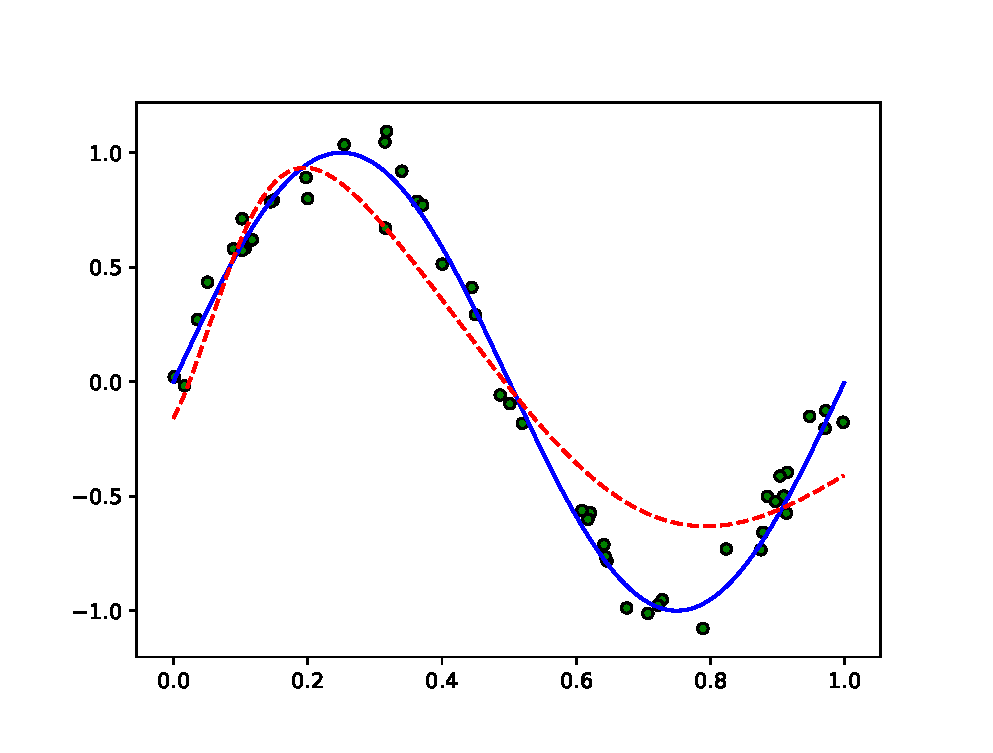
\includegraphics[width=0.75\textwidth]{prediction.eps}
	\caption{Juxtaposition of the noisy data points, the noiseless sinewave they are based on, and the manifold of the stochastic gradient descent regression model.}
\end{figure}

\begin{figure}[H]
	\centering
	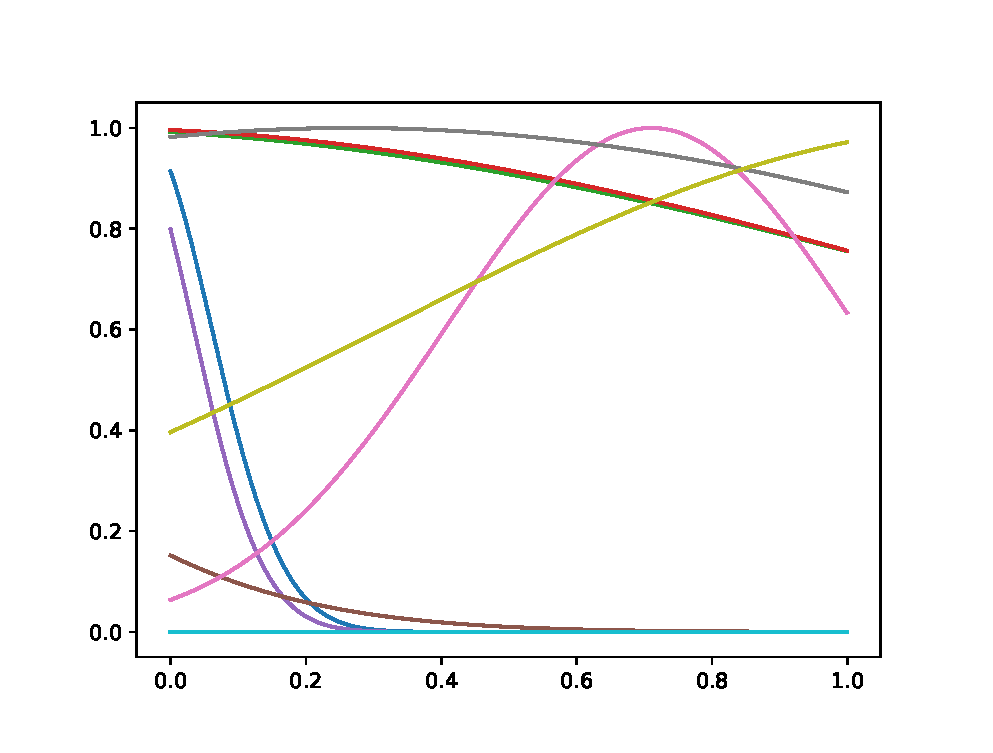
\includegraphics[width=0.75\textwidth]{bases.eps}
	\caption{A plot of each of the basis functions, with the weights and intercept removed.}
\end{figure}

\clearpage
\begin{adjustwidth}{-50pt}{0pt}

\section{Code}

\begin{Verbatim}
import numpy as np
import tensorflow as tf
import matplotlib.pyplot as plt
from tqdm import trange

# M
NUM_FEATURES = 10

# n
NUM_SAMP = 50

BATCH_SIZE = 32
NUM_BATCHES = 300
LEARNING_RATE = 0.1
SIGMA_NOISE = 0.1
np.random.seed(31415)
tf.random.set_seed(31415)

class Data(object):
	def __init__(self, num_samp=NUM_SAMP, num_features = NUM_FEATURES):
	"""
	Draw random weights and bias. Project vectors in R^NUM_FEATURES
	onto R with said weights and bias.
	"""
	num_samp = NUM_SAMP
	sigma_noise = SIGMA_NOISE
	
	
	self.index = np.arange(num_samp)
	
	self.x = np.random.uniform(low = 0, high = 1, size = (num_samp, 1))
	self.epsilon = np.random.normal(loc = 0, scale = sigma_noise, size = (num_samp, 1))
	self.y = np.sin(2*np.pi*self.x) + self.epsilon
	
	def get_batch(self, batch_size=BATCH_SIZE):
	"""
	Select random subset of examples for training batch
	"""
	choices = np.random.choice(self.index, size=batch_size)
	
	return self.x[choices].flatten(), self.y[choices].flatten()


class Model(tf.Module):
	def __init__(self, num_features=NUM_FEATURES):
		"""
		A plain linear regression model with a bias term
		"""
		self.w = tf.Variable(tf.random.normal(shape=[num_features, 1]))
		self.mu = tf.Variable(tf.random.normal(shape=[num_features, 1]))
		self.sigma = tf.random.normal(shape=[num_features, 1])
		self.b = tf.Variable(tf.zeros(shape=[1, 1]))
	
	def __call__(self, x):
		return tf.squeeze(tf.transpose(self.w)
			@ tf.exp(-tf.square(x - self.mu)/(tf.square(self.sigma))) + self.b)

if __name__ == "__main__":
	data = Data()
	model = Model()
	optimizer = tf.optimizers.SGD(learning_rate=LEARNING_RATE)
	
	bar = trange(NUM_BATCHES)
	for i in bar:
		with tf.GradientTape() as tape:
			x, y = data.get_batch()
			y_hat = model(x)
			loss = tf.reduce_mean(0.5*((y_hat - y) ** 2))
		
		grads = tape.gradient(loss, model.variables)
		optimizer.apply_gradients(zip(grads, model.variables))
		
		bar.set_description(f"Loss @ {i} => {loss.numpy():0.6f}")
		bar.refresh()
	
	w_hats = np.squeeze(model.w.numpy())
	b_hat = np.squeeze(model.b.numpy())
	sigma_hats = np.squeeze(model.sigma.numpy())
	mu_hats = np.squeeze(model.mu.numpy())
	
	PLOT_MARKER_SIZE = 25
	
	x = np.arange(0, 1, 0.001)
	y = np.sin(2*np.pi*x)
	y_model = model(x)
	
	fig1, ax1 = plt.subplots()
	
	noiseless_sine = ax1.plot(x, y, c = "blue")
	noisy_data = ax1.scatter(data.x,
		data.y,
		s = PLOT_MARKER_SIZE,
		c = "green",
		edgecolors = "black")
	trained_model = ax1.plot(x, y_model, '--', c = "red")
	
	fig1.savefig("prediction.png")
	fig1.savefig("prediction.eps")
	
	fig2, ax2 = plt.subplots()
	x2 = np.arange(-5, 5, 0.1)
	for w_hat, sigma_hat, mu_hat in zip(w_hats, sigma_hats, mu_hats):
	phi = tf.squeeze(tf.exp(-1*(x - mu_hat)**2/((sigma_hat)**2)))
	plt.plot(x, phi)
	
	fig2.savefig("bases.png")
	fig2.savefig("bases.eps")
	
	print("w_hat")
	for w_hat, sigma_hat, mu_hat in zip(w_hats, sigma_hats, mu_hats):
	print("w_hat, sigma_hat, mu_hat, b_hat\n")
	print(f"{w_hat:0.2f}, {sigma_hat:0.2f}, {mu_hat:0.2f}, {b_hat:0.2f}")
\end{Verbatim}
\end{adjustwidth}

\end{document}